%2multibyte Version: 5.50.0.2960 CodePage: 936
%\usepackage{subfig}
%\usepackage{bbm}
%\hypersetup{hidelinks} % hide the ugly red box in footnote links
%\setcitestyle{authoryear,round}
%\doublespacing
%\graphicspath{{figure/}}
% defines ExpandableInput command which solves the
% problem of having noalign problem in the first line
% of input tables
% defines
% the superscripts in tables (significance stars)
\documentclass[12pt]{article}
\usepackage{eurosym}
\usepackage{rotating}
\usepackage{amsmath}
\usepackage{graphicx}
%\usepackage{subfig}
\usepackage{verbatim}
\usepackage{caption}
\usepackage{subcaption}
\usepackage{setspace}
\usepackage{color}
\usepackage{amsfonts}
\usepackage{amssymb}
\usepackage{float}
\usepackage{ulem}
\usepackage{soul}
%\usepackage{bbm}
\usepackage[authoryear,round]{natbib} % 文献
\usepackage{hyperref}
\usepackage{makecell}
\usepackage[toc,page,header]{appendix}
\usepackage{minitoc}
%\hypersetup{hidelinks} % hide the ugly red box in footnote links
\setcounter{MaxMatrixCols}{10}
\providecommand{\U}[1]{\protect\rule{.1in}{.1in}}
\pagestyle{plain}
\hypersetup{hypertex=true,
colorlinks=true,
linkcolor=blue,
anchorcolor=blue,
citecolor=blue}
%\setcitestyle{authoryear,round}
\usepackage[margin=1truein]{geometry}
\newtheorem{theorem}{Theorem}
\newtheorem{acknowledgement}[theorem]{Acknowledgment}
\newtheorem{algorithm}{Algorithm}               
\newtheorem{axiom}{Axiom}
\newtheorem{case}{Case}
\newtheorem{claim}{Claim}
\newtheorem{conclusion}{Conclusion}
\newtheorem{condition}{Condition}
\newtheorem{conjecture}{Conjecture}
\newtheorem{corollary}{Corollary}
\newtheorem{criterion}{Criterion}
\newtheorem{definition}{Definition}
\newtheorem{example}{Example}
\newtheorem{exercise}{Exercise}
\newtheorem{lemma}{Lemma}
\newtheorem{notation}{Notation}
\newtheorem{problem}{Problem}
\newtheorem{proposition}{Proposition}
\newtheorem{remark}{Remark}
\newtheorem{solution}{Solution}
\newtheorem{summary}{Summary}
%\doublespacing
\onehalfspacing
\newenvironment{proof}[1][Proof]{\textbf{#1.} }{\ \rule{0.5em}{0.5em}}
\RequirePackage{threeparttable}
\RequirePackage{booktabs}
\RequirePackage{tabularx}
\graphicspath{{figure/}}
\makeatletter\let\ExpandableInput\@@input\makeatother
% defines ExpandableInput command which solves the
% problem of having noalign problem in the first line
% of input tables
\def\sym#1{\ifmmode^{#1}\else\(^{#1}\)\fi}  % defines
% the superscripts in tables (significance stars)
\input{tcilatex}
\begin{document}

\title{Does Pollution Affect Exports? -- Evidence from China\thanks{%
Thanks note here...}}
\author{Jie Bai\thanks{%
Department of Economics, Lingnan University, Hong Kong, E-mail: jiebai@ln.hk}
\quad Larry D. Qiu\thanks{%
Department of Economics, Lingnan University, Hong Kong, E-mail:
larryqiu@ln.edu.hk} \quad Junji Xiao\thanks{%
Department of Economics, Lingnan University, Hong Kong, E-mail:
junjixiao@ln.edu.hk. \copyright\ 2022 Jie Bai, Larry D. Qiu and Junji Xiao.
All Rights Reserved. }}
\date{September 10, 2022}
\maketitle

\begin{abstract}
  Trade is an important driving force for rapid economic growth but almost
  inevitably accompanied by deterioration in environment, especially in
  developing countries. In contrast to existing studies that investigate the
  impact of trade on environment, this paper analyzes the reverse effects,
  that is, whether pollution affects exports and if yes, how, by examining the
  Chinese export and pollution data over the period of 2000--2007. Using $%
  \mathrm{PM_{2.5}}$ concentrations as a proxy for air pollution, we estimate
  the causal effect of air pollution on the Chinese firms' exports, employing
  thermal inversion as an instrument variable. We find that an 1\% increase in 
  $\mathrm{PM_{2.5}}$ leads to an 1.09\% reduction in firm-level exports. This
  reduction in exports is mainly attributed to the intensive margins as
  opposed to the extensive margins. The mechanism analysis suggests
  coexistence of two channels: air pollution adversely affects productivity
  and also invites stringent environmental regulations, both reducing exports.
  \end{abstract}
  \begin{quote}
    \emph{Keywords:} Export; Air Pollution; Productivity; Environmental
    Regulation
    \end{quote}
    \begin{quote}
    \emph{JEL Classification:} F14, F18, Q51
    \end{quote}
    \newpage
    \setcounter{page}{1}
    \section{Introduction}

    \label{sec:1} The rapid trade economic growth is usually accompanied by
environmental deterioration especially in developing countries such as
China. From 1998 to 2007, air quality in China deteriorated substantially.
For example, the \textcolor{red}{annual average} $\mathrm{PM_{2.5}}$ concentration increased from
32.32 $\mu g/m^{3}$ to 49.18 $\mu g/m^{3}$. The \textcolor{red}{annual mean} concentration exceeds
the WHO air quality guidelines every year, causing concerns about the
balance of environment and economic development.\footnote{%
For fine particulate matter ($\mathrm{PM_{2.5}}$), WHO published guideline
values for 5 $\mu g/m^{3}$ annual mean and 15 $\mu g/m^{3}$ 24-hour mean.
See %
\url{https://www.who.int/news-room/fact-sheets/detail/ambient-(outdoor)-air-quality-and-health}
for more information.} [\textbf{Question}: according to the footnote, there
are two types of mean. Which one did you report above?] Empirical evidences
have shown that severe pollution reduces labor productivity through
influencing people's health both physically and mentally as health is a very
important part of human capital %
\citep{graff2012impact,chang2016particulate,zhang2018impact,fu2021air,somanathan2021impact,adhvaryu2022management}%
. In this paper, we ask a different but related question: does pollution
influence international trade and how? We examine this question based on the
evidence of China, which experienced rapid increases in both trade and
pollution.

There exists a large literature of the impacts of trade on environment.%
\footnote{%
See \cite{cherniwchan2017trade} for the most recent survey of the literature.%
} However, studies on the impacts of environment on trade are rare. As
common, a biggest challenge in the empirical studies of trade and
environment is the endogeneity problem. This problem is more serious in the
estimation of the effects of pollution on trade than that of trade on
pollution, because in the latter case, researchers often find good
instrumental variables for trade, such as trade agreements and trade shocks.
In this study, we overcome the endogeneity problem using the instrumental
variable method to examine the causal impact of air pollution on firms'
exports. In particular, we follow the literature \citep{fu2021air, fu2021trans,NBERw28401,chen2022effect} [\textcolor{red}{I add one citation (Fu et al.2021)  }] to use both thermal inversions and
wind directions as instrumental variables for an important type of air
pollution, i.e., $\mathrm{PM_{2.5}}$ concentrations, at county level, to
study the effects of pollution on firms' exports in China from 2000 to 2007. 

Our empirical findings suggest that exports decrease as $\mathrm{PM_{2.5}}$
levels increase. Specifically, following a 1\% increase in $\mathrm{PM_{2.5}}
$ concentration, the average exporter decreases its export value by 1.09\%.
Air pollution also influences firms' exporting decisions: an 1\% increase in 
$\mathrm{PM_{2.5}}$ concentration reduces a firm's probability of entering
foreign markets by 0.06 percentage point and raises an exporter's
probability of exiting foreign markets by 0.15 percentage point. We also
find that air pollution has detrimental effects on labor productivity and
total factor productivity (TFP), echoing the findings in the existing
literature \citep{NBERw18392,fu2021air,NBERw28401}.
This suggests that reducing productivity is a channel through which air
pollution reduces exports. In addition, we find that the negative effect of
air pollution on exports is significant only in the regions with
government-specified pollution abatement targets. This finding suggests
another channel: governments in pollution-intensive regions impose more
stringent control on pollution, raising the costs of production and so
undermining the firms' competitiveness in exports. This last finding
provides additional evidence supporting the previous studies on how
environmental regulations affect individual firms' exports %
\citep{cherniwchan2022environmental}. [\textbf{NOTE}: please revise this
reference: change the capital letters of the title to small letters. we
should also include the working paper no. Also check other reference
entries: not consistent in using capital letters and small letters, for
example: Journal of development economics. china, Wto, etc.]

This paper makes a significant contribution to the literature of
international trade and environment. Several review articles of this
literature are available including \cite{cherniwchan2017trade} and \cite%
{NBERw30020} as the most recent ones. Almost all existing
studies focus on how international trade affect pollution. A general
conclusion is that trade liberalization (and therefore trade) alters
emissions (or more generally, pollution) via scale, composition, and
technique effects \citep{NBERw3914,copeland1994north}.
The composition effect receives particular attention as it is related to the
pollution haven hypothesis, that is, pollution-intensive industries
\textquotedblleft move\textquotedblright\ to countries with lax
environment policies \citep{copeland1994north,taylor2005unbundling}. Our
paper clearly differs from this strand of literature as we examine the
opposite direction of the effects: how pollution affects trade.

Although they are scant, a few studies exist in examining the effects of
environmental factors on trade. \cite{jones2010climate} [\textbf{NOTE}: this
paper is not listed in the References. Please check the match: whether all
cited papers are included in the References and whether all papers in the
References are cited in our paper.] find that higher temperatures in poor
countries lead to large, negative impacts on the growth of their exports,
mainly in agricultural exports and light manufacturing exports. \cite%
{dellink2017international} verbally describe the potential channels through
which climate change damages affect trade. The channels include the direct
impact on transport and distribution chains, and the indirect influences on
factors of production. Unlike these papers, we conduct a rigorous empirical
analysis of the effects of air pollution on exports, based on firm-level
data. Thus, our study is a valuable addition to this strand of literature.

As mentioned earlier, the mechanisms that work in our finding of the
pollution effects on exports are productivity and environmental regulations.
This part of study in our paper is closely related to two literatures. The
first is the effects of pollution on productivity. \textcolor{red}{There is a large body of literature that provide convinced evidences causally linking various air pollution (i.e. ozone, $\rm PM_{2.5}$) to productivity in different sectors. They all show the negative relationship between pollution and productivity \citep{graff2012impact,chang2016particulate,fu2021air,adhvaryu2022management}. } [\textbf{To be added}]
Our finding is consistent with the general conclusion of this literature.

The second literature is the effects of enviromental regulations on exports.

[\textbf{NOTE to myself}: I need to understand how we estimate productivity
first. If productivity has include abatement cost, then both pollution and
regulation affect productivity jointly, rather than pollution affects
productivity as one channel and regulation affects cost as another.]

Our study is also related to a small literature on the impacts of
environmental regulations and policies on various economic outcomes,
especially on productivity and trade. The effects of environmental
regulations on productivity are mixed. \cite{berman2001environmental} find
that TFP rises in air quality regulation regions as abatement investment
appear to be productivity enhancing in the US. \cite{NBERw18392}
find stricter air quality regulations are associated with a roughly 2.6
percent decline in TFP in the US. \cite{he2020watering} find that a water
quality regulation campaign in China significantly reduces upstream
polluting firms TFP by more than 24\% compared to downstream. They link this
water quality regulations to political evaluations. Therefore, local
government officials were more incentive to tighten the water quality
standards of upstream of monitor stations.

A few recent papers explore the environmental regulations and their
influences on trade.\footnote{%
Some papers investigate the effects of environmental regulations on foreign
direct investment \citep{dean2009foreign,cai2016does}.} \cite{%
hering2014environmental} study the Two Control Zones policy in China and
find that exports significantly reduce in targeted cities and sharper fall
for pollution-intensity industries. \cite{shi2018environmental} show that
pollution reduction targets in China's Eleventh Five-Year Plan result in
exports fall in targeted cities. Different from these studies, our paper
focuses on the effects of pollution \textit{per se} on exports.

The rest of the paper is orgnanized as follows. We specify our empirical
strategy in Section 2. We describe our data and
measurements in Section 3. We present the main empirical findings in Section
4 and explore the mechanisms in Section 5. We provide concluding remarks in
Section 6.

\section{Empirical Model and Identification}

\label{sec:empirical_strategy} This section presents our empirical
methodology of estimating the impact of air pollution on individual firms'
exports. \sout{Two stage least squares (TSLS)} \textcolor{red}{Two-Stage least squares (2SLS)} [\textcolor{red}{Question: should we use "2SLS" for it's more common and popular used among recent reduce-form paper and econometrics?}]estimation is applied to solve the
potential endogeneity problem with pollution.

\subsection{Empirical Model}

To investigate the impact of air pollution on firms' exports, we assume
exports to be a function of pollution; moreover, we control for the major
determinants of exports following previous literature %
\citep[e.g.,][]{kunst1989exports,bernard2003plants}. Specifically, letting $Export_{ict}$
denote the value of exports by firm $i$ from county $c$ in year $t$, we
assume 
\begin{equation}
Log(Export_{ict})=\beta _{0}+\beta _{1}Log(P_{ct})+\mathbf{X}%
_{ict}^{^{\prime }}\Gamma +\mathbf{W}_{ct}^{^{\prime }}\beta _{w}+\delta
_{i}+\lambda _{t}+\epsilon _{ict}.  \label{equ1}
\end{equation}%
In the above equation, $log(Export_{ict})$ is the \textcolor{red}{natural} logarithmic value of
exports. $Log(P_{ict})$ is the logarithmic air pollution density. The vector 
$\mathbf{X}_{ict}^{^{\prime }}$ consists of variables measuring the firm
characteristics, including age, size, total capital, and productivity.
Productivity is measured by either labor productivity or revenue-based TFP.
Labor productivity is defined as the ratio of the firm's value added to the
number of employees. We estimate TFP using both Levinsohn-Petrin method %
\citep{levinsohn2003estimating} and Olley-Pakes method %
\citep{olley1996dynamics}, denoted as $TFP_{LP}$ and $TFP_{OP}$,
respectively. TFP is estimated using the output data at two-digit Chinese
Standard Industrial Classification (CSIC), considering heterogeneous
productivity across industries. All measures of productivity are in
logarithmic form and are deflated by respective price index developed by %
\citep{brandt2017wto}. As the previous literature %
\citep[e.g.,][]{jones2010climate} suggests that weather may affect exports,
we also control for weather, represented by vector $\mathbf{W}%
_{ct}^{^{\prime}}$, which includes temperature, precipitation, humidity,
wind speed, and sunshine duration. $\lambda _{t}$ is the time fixed effects,
capturing the time trends and all other possible time-specific shocks such
as annual socioeconomic cycles that may affect exports. \sout{$\delta _{i}$ is the
firm fixed effects, which is time-invariant, capturing firm-specific
unobservable characteristics contributing to exports.} \textcolor{red}{Since few
firms switch industries, so all time-invariant, industry-specific
unobservable affecting exports are absorbed by the firm fixed effects $\delta _{i}$.} \sout{$\epsilon _{ict}$ is
the error term, which is assumed to be mean zero and independent across
firms, allowing within-firm auto correlation.} \textcolor{red}{The error term $\epsilon _{ict}$ is clustered at firm-level, allowing to correlate within the same firm.}

We list the definitions of the key variables in Table~\ref{tab:var_definition} for easy reference.

\begin{center}
$<$Table~\ref{tab:var_definition} Here$>$
\end{center}

\subsection{Identification \textcolor{red}{Strategy: Instrument Variable}}

\sout{One concern with this model identification is the endogeneity problem of
pollution: The determinants of exports affect firms' outputs and so the
emission of pollutants, resulting in a correlation between the independent
variable $Log(P_{ct})$ and the error term $\epsilon _{ict}$. Intuitively,
the increased exports and deteriorated environment could be the simultaneous
consequence of positive shocks to production. This endogeneity problem makes
ordinary least sqaures (OLS) estimators biased.} \footnote{%
\sout{The OLS estimator could suffer from upward or downward bias. For example,
certain firms may upgrade their production technology over time and adopt
energy-saving and environmentally friendly technology. In this scenario, low
pollution and high exports are observed, attenuating the negative effects of
pollution on exports and so leading to upward bias. In the contrary, certain
firms may have insufficient funds to upgrade their production technology
over time. In this scenario, OLS estimator generates downward bias. Local
environmental regulations may also bias the OLS estimators. Regions with
more exports usually observe faster economic growth at the cost of
pollution. In response, the local governments may impose more stringent
environmental regulations, leading to low pollution but high production
costs and so low exports} \citep{cherniwchan2022environmental,shi2018environmental}; \sout{as a consequence,
the OLS estimator will also suffer from downward bias.}} 

\textcolor{red}{However, the OLS estimation applied to Eq.(\ref{equ1}) will be biased, due to endogeneity problems: reverse causality and omitted variable bias. For instance, the increased exports and deteriorated environment can simultaneously interact. Or the omitted factors such as new production technology or other characteristics can simultaneously affect export and air quality. }[\textbf{Question}:
Should we also talk about the causality problem here? \textcolor{red}{I agree but I am confused about the sentence "The determinants of exports affect firms' outputs and so the emission of pollutants, resulting in a correlation between the independent
variable $Log(P_{ct})$ and the error term $\epsilon _{ict}$" how the determinants of exports affect the emission of pollutants? There are two main endogeneity problem: 1. export and pollution are reverse causality 2. confounding factors that both influence export and pollution but are omitted. The deleted sentences only talked about reverse causality problem.}] \sout{To address this
problem, we use an IV for $log(P_{ct})$ and apply the TSLS estimation to
Model (\ref{equ1}).} \textcolor{red}{To address these endogenous challenges, we adopt an IV strategy.} Following the literature of environmental economics %
\citep{arceo2016does,jans2018economic,sager2019estimating,fu2021air,NBERw28401}%
, we use county-level days of thermal inversions per annum as the
instrumental variable. In the first stage of the \sout{TSLS} 2SLS, we regress pollution
on TI, controlling for the variables as in Model~(\ref{equ1}) and get the
fitted value of $Log(P_{ct})$ to be used for the second stage of the \sout{TSLS} 2SLS.

As described by \cite{jacobson2002atmospheric}[\textbf{NOTE}: include this paper in the
Reference: Jacobson, M. (2002). Atmospheric Pollution. History, Science, and
Regulation, Cambridge: Cambridge University Press.] and \cite{arceo2016does},
thermal inversion is a reversal of the normal behaviour of temperature in
the troposphere, which is the region of the atmosphere nearest Earth's
surface. Under normal conditions air temperature usually decreases with
height. When a layer of cool air at the surface of the troposphere is
overlain by a layer of warmer air, which acts as a cap on the upward
movement of the air from the layers below, a thermal inversion occurs (see
Fig.~\ref{fig:1}). Consequently, convection caused by the heating of the air
from below is limited to levels below the inversion and so air pollution is
trapped close to the ground due to thermal inversion. This positive
correlation between air pollution and thermal inversion is owing to
meteorological factors.

\begin{center}
  $<$Figure~\ref{fig:1} Here$>$
  \end{center}
  
  Thermal inversion occurs for three \textcolor{red}{typical} reasons. First, a \sout{subsidence} inversion
  occurs when there is a high pressure system and air from high pressure
  center in the atmosphere sinks down to fill the space left as air blows
  outward, resulting in a layer of hot air on a layer of cold. Second, thermal
  inversion can happen when air moves horizontally and a warm air layer is
  squeezed upwards onto the cold denser air. Third, a \sout{radiation} inversion
  happens when air temperature near the ground cools down faster than that in
  the air above, resulting in the temperature near the ground lower than that
  in the upper layers. [\textbf{NOTE}: I don't understand the logic of this
  paragraph. We say TI occurs for three reasons at the begining, but then the
  first is about subsidence inversion and the last is about radiation
  inversion. What are their relation to TI? \textcolor{red}{inversion caused by subsidence process are called subsidence inversion; caused by ground radiation called radiation inversion.}]
  
  Because thermal inversion is a pure meteorological phenomenon which affects
  pollution but is unlikely to directly affect other economic and social
  activities, it has become a popular instrumental variable for pollution in
  empirical studies %
  \citep{arceo2016does,jans2018economic,sager2019estimating,chen2022effect,NBERw28401}%
  . It is also a valid \sout{intromental} \textcolor{red}{instrumental} variable in our study because it satisfies
  the following three conditions[\textcolor{red}{NOTE: For a valid IV, need to satisfy \textbf{two conditions} referring to econometrics papers. relevance(correlation); exogeneity(exclusion)}].: Relevance, exogeneity and exclusion. First,
  as we describe above, when a thermal inversion occurs, pollutants are
  trapped in the air close to the ground, and thus, pollution level increases.
  Hence, a number of thermal inversions observed in a year is positively
  correlated with the average pollution level of the year. The relevance
  condition is satisfied. We confirm this positive correlation later based on
  our data of thermal inversions and $\mathrm{PM_{2.5}}$ at county-year level
  in China.
  
  \  Second, no evidence suggests that thermal inversions are correlated with
  exports. Thermal inversions are driven by meteorological factors but not by
  socioeconomic factors, and so they not correlated with economic activities
  such as exports. Hence, our instrumental variable satisfies the \sout{endogeneity
  condition} \textcolor{red}{exclusion restriction}. We confirm this later with the evidence based on our data of
  thermal inversions at county-year level in China. Third, as discussed
  previously [\textbf{Question}: where exactly? \textcolor{red}{I don't know either. There is no need a third condition as a valid IV}], the only channel through
  which thermal inversions may affect exports is through pollution. 

    \section{Data and Measurement}

    \label{sec:3}
    
    \subsection{Pollution}
    
    \label{sec:3.1} Our study focuses on air pollution. There exist different
    measures for air pollution. The US Environmental Protection Agency has
    identified six pollutants as \textquotedblleft criteria\textquotedblright\
    air pollutants, including carbon monoxide, lead, nitrogen oxides,
    ground-level ozone, particle pollution (often referred to as particulate
    matter), and sulfur oxides. These pollutants are found to harm human health
    and the environment. Among these pollutants, the particulate pollutant that
    is 2.5 microns or smaller in size, or $\mathrm{PM_{2.5}}$, is widely used in
    the literature as an index for air pollution %
    \citep{chang2016particulate,fu2021air,NBERw28401}. Following this literature, we also
    use $\mathrm{PM_{2.5}}$ concentration to measure air pollution.
    
    We use the satellite-based $\mathrm{PM_{2.5}}$ concentrations constructed
    and estimated by \cite{van2021monthly} in our study.\footnote{\cite%
    {van2021monthly} estimate fine particulate matter ($\mathrm{PM_{2.5}}$) by
    combining Aerosol Optical Depth (AOD) retrievals from the NASA MODIS, MISR,
    and SeaWIFS instruments with the GEOS-Chem chemical transport model, and
    subsequently calibrating to global ground-based observations using a
    Geographically Weighted Regression (GWR) at high grid resolution. The Global
    Annual $\mathrm{PM_{2.5}}$ Grids data is available on the website of the
    Atmospheric Composition Analysis Group at Washington University in St. Louis
    (\url{https://sites.wustl.edu/acag/datasets/surface-pm2-5/}).}  The
    concentrations are available at a spatial resolution of 0.01-by-0.01-degree
    latitude-longitude grid of the GIS raster (approximately 1.11 kilometers by
    1.11 kilometers). To the best of our knowledge, this is the finest
    resolution for the concentration data. This satellite-based data has a few
    advantages over ground-based pollution data from official sources. First,
    the satellite-based $\mathrm{PM_{2.5}}$ cover all counties, the smallest
    administrative unit in China, and are available from 1998, whereas the
    official $\mathrm{PM_{2.5}}$ data are only available for large cities since
    2012.\footnote{%
    On February 29, 2012, the State Council of China firstly agreed to issue the
    newly revised Ambient Air Quality Standards. The new standard adds
    monitoring indicators for fine particulate matter ($\mathrm{PM_{2.5}}$) and
    ozone ($O_{3}$ ). Therefore, the official data of $\mathrm{PM_{2.5}}$
    concentration was not available until then.} Second, official air quality
    data may be potentially manipulated by local officials before publication %
    \citep{ghanem2014effortless,andrews2008inconsistencies}, because local
    environmental quality has become a vital criterion for government officials
    \^{a}\euro \texttrademark\ promotion evaluation since 2006 and particularly
    after 2015 \citep{fan2022unintended}.
    
    We aggregate grid-level $\mathrm{PM_{2.5}}$ concentrations to county level. \textcolor{red}{For each year, we calculate the county's average $\rm PM_{2.5}$ concentrations as the mean of values of all grid cells that overlapping
    the county.}
    \sout{Specifically, we obtain a county's annual $\mathrm{PM_{2.5}}$ concentration
    using the mean value of $\mathrm{PM_{2.5}}$ concentrations from all grid
    cells within the county.} [\textbf{NOTE}: However, you have not describe how
    to obtain the \textbf{annual} concentration of each \textbf{grid}. \textcolor{red} {This raw data: satellite-based PM2.5 value is Annual for each grid. The footnote describes it "Global Annual PM2.5 Grids data".}] Fig.~%
    \ref{fig:3} presents the map of county-level average concentration of $%
    \mathrm{PM_{2.5}}$ over the period 1998--2007 in China. There exist
    substantial spatial variations of $\mathrm{PM_{2.5}}$ concentrations across
    counties, ranging from 1.33 $\mu g/m^{3}$ to 97.57 $\mu g/m^{3}$. [\textbf{%
    NOTE}: I don't find the following statements convincing and helpful. Should
    delete it: \sout{The northeastern and eastern regions and southern Xinjiang
    areas, an autonomous territory in northwest China, suffer from more severe
    air pollution. As most of these areas also observe higher economic growth
    rates than the other inland areas during the same period}] The spatial heterogeneity in air pollution could be
    attributed to differences in physiographic and meteorological conditions
    across regions on the one hand, and also to the differences in regional
    socioeconomic factors such as economic activities and environmental
    regulations on the other hand. The large variations of $\mathrm{PM_{2.5}}$
    concentrations give us the opportunity to explore the pollution effects on
    economic activities such as exports. 
    
    \begin{center}
    $<$Figure~\ref{fig:3} Here$>$
    \end{center}

    \subsection{Thermal Inversions and Weather}

\label{sec:data_TI} Thermal inversion is an phenomenon of air temperature at
the near ground second layer being higher than the first layer. To measure
the occurence of thermal inversions, we exploit the vertical temperature
data from NASA Modern-Era Retrospective Analysis for Research and
Applications (Version 2, or MERRA-2).\footnote{%
This dataset is titled M2I6NPANA and available at %
\url{https://disc.gsfc.nasa.gov/datasets/M2I6NPANA_5.12.4/summary}.} This
data set provides 6-hour air temperature at 42 atmospheric layers at a grid
level of 0.5 
%TCIMACRO{\U{b0} }%
%BeginExpansion
${{}^\circ}$
%EndExpansion
by 0.625 
%TCIMACRO{\U{b0} }%
%BeginExpansion
${{}^\circ}$
%EndExpansion
(about 45km by 55km in terms of distance). For each grid cell, we compare
the air temperature in the ground atmospheric layer (in the surface measure
conditions of 1000 Hectopascal pressure unit (hPa), which is around 110
meters above sea level), called layer 1, with that in the second atmospheric
layer close to ground (in the measure conditions of 975 hPa, approximately
320 meters above sea level), called layer 2.\footnote{%
Sometimes we observe missing temperatures at low air pressure levels because
the altitude of the land surface is high in that grid. In those cases, we
label the atmospherical layers based on their relative hight to the surface,
rather than using the uniform air pressure levels. As a result, layer 1
always corresponds to the lowest air pressure level above the surface.}
Under normal conditions, temperature decreases with altitude. If on a
particular day we observe that layer 1's temperature higher than layer 2's
temperature, then we say thermal inversion occures on that day. We obtain
the measure of thermal inversions of each grid cell using the number of days
with thermal inversions occurrence in that grid cell in a year. \textcolor{red}{Then, we aggregated at county level
using a weighted average (by area) across all grids that it spans.}[\textbf{NOTE%
}: I don't understand the following description: Then, we \textbf{aggregate}
the grid level TIs to the county average using the cell areas spanning the
county as \textbf{weights}. \textcolor{red}{grid cells may be split by county boundary, I give more weights to those grid span more in a county.}] In the robustness check, we define another
measure of thermal inversions by comparing air temperature differences
between the ground and third-close-to-ground (the 950hPa layer, which is
around 540m above sea level) layers.

We obtain station-level daily weather indicators from National
Meteorological Information Center of China. In particular, we make use of
the dataset is provided by National Tibetan Plateau Data Center %
\url{(http://data.tpdc.ac.cn)}, which contains daily basic meteorological
variables including air temperature, precipitation, relative humidity, wind
direction and speed, sunshine duration and barometric pressure, collected
from 699 national meteorological stations in China since year 1951 %
\citep{Dailymeteorologicaldataset}. For each county, we use
Inverse-Distance-Weighting (IDW) method to convert the station-level
observations into county-level data, assigning lower weights to the stations
further away from the county center. Temperature is a key indicator of
weather. We use a vector of temperature distribution as the temperature
variable of each county. \textcolor{red}{To
include the nonlinear effects of weather, we calculate 20 quantiles of the overall daily distribution of temperature variable and calculate the share of days in a year that fall into each of the 20 quantiles following \citep{deschenes2017defensive}.}[\textbf{NOTE}: I don't understand the following
description: Taking into account the nonlinear effects of weather as
proposed by \citep{deschenes2017defensive}, we divide the sample
distribution of temperature into twenty equal-size quantiles and then count
the frequency of the daily temperature (the number of days) falling in these
quantiles for each county each year. In this way, we generate a
twenty-dimensional vector recording the frequency distribution of the
county's temperature.] [\textbf{Question}: which papers use such type of
temperature variable?\textcolor{red}{\citep{deschenes2017defensive} this paper use such weather controls because extreme weather events have differential effects from more normal ones.}] \textcolor{red}{Twenty temperature bins, together with the \sout{squared terms} \textcolor{red}{second-degree polynomials} of precipitation, humidity, wind speed,
and sunshine duration, respectively, as weather controls in $\mathbf{W}_{ict}^{^{\prime }}$ Model (1) \citep{chen2022effect}.} [\textbf{Question}%
: why using squared terms rather than distribution like temperature? Some
explanations.\textcolor{red}{The effect of weather is nonlinear, so that both 20 bins and polynomials can capture this nonlinear effect. From literature, some use bins/polynomials or they are mixed used. Here is more like technical trick in data generating process. This combination of weather control is more adopted to this data.}] \sout{All these individual variables together form the weather
vector in $\mathbf{W}_{ict}^{^{\prime }}$ Equ.(1).}

With the above constructions of county-level $\mathrm{PM_{2.5}}$
concentrations and thermal inversions, we can now explore their correlations
and time trends, which are presented in Fig.~\ref{fig:3}. The top panel
shows a strong positive correlation between thermal inversions and $\mathrm{%
PM_{2.5}}$ concentrations: counties that had high average thermal inversions
over 1998--2007 also had high average $\mathrm{PM_{2.5}}$ concentrations
over the same period. This is a supporting evidence of thermal inversions'
satisfaction of the relevance condition for a valid instrumental variable,
as argued earlier. 

The bottom panel shows the time trends of thermal inversions and $\mathrm{%
PM_{2.5}}$ over the period of 1998--2007. First, there is no obvious time
trend of thermal inversions, which is largely consistent with the definition
of thermal inversions being \sout{an} \textcolor{red}{a} meteorological \sout{phenonenon} \textcolor{red}{phenomenon} not related to
economic activities.\sout{and pollution} \textcolor{red}{[NOTE: thermal inversions is positively correlated with air pollution]}. This is a supporting evidence of thermal
inversions' satisfaction of the exogeneity condition for a valid
instrumental variable, as argued earlier. 

[\textbf{Question}: Any additional information this can provide compared to
the top panel? Moreover, the two curves of PM2.5 imply an increasing time
trend, which is true. But this may creat unncesarry question: TI is random
(no time trend) but PM2.5 has time trend, then are they positively
correlated? Think more carefully about this. \textcolor{red}{TI is systematically random but average PM2.5 increased over years which would not be a violation to their positive correlation. It can be observed that although the average PM2.5 of counties increased as time goes by (the overall decreased in air quality), large variations of PM2.5 exist across counties. we can see areas with higher pollution have higher TI frequencies. the additional information should be the following sentence.}] $\mathrm{PM_{2.5}}$
concentrations the air pollution is systematically higher in the areas with
high frequencies of thermal inversions than in the areas with low frequencies of thermal inversions, also suggesting a
positive correlation between thermal inversions occurrence and $\mathrm{PM_{2.5}}$
concentrations.


\subsection{Firm-level Data}

\label{sec:data_firm} The firm characteristics are calculated based on data
collected from the Annual Survey of Industrial Firms (ASIF) by China's
National Bureau of Statistics. The ASIF dataset covers all firms with annual
sales above RMB 5 millions in China from 1998 to 2013. In total, there are
over 1.4 million observations for around 430 thousand firms over all
provinces in China. Following the literature \citep[e.g.,][]{fu2021trans}[\textcolor{red}{QUESTION: Is this cite appropriate? We all know that focusing on manufacture sector is a common practice in trade analysis. If we have to cite,\cite{brandt2012creative} may be more precise?}],
we focus on firms in the manufacturing sector in empirical analysis.

The ASIF data provide detailed information of each firm's balance sheet,
such as gross output, value added, employment, capital, intermediate inputs,
and ownership. To correct the potential errors from data input, we drop the
abnormal observations that violate the following Generally Accepted
Accounting Principles: liquid assets are greater than total assets, total
fixed assets are greater than total assets, the net value of fixed assets is
greater than total assets, and current depreciation [\textbf{Question}:
depreciation of what? \textcolor{red}{In ASIF data, current depreciation and accumulated depreciation are not specified to which item, I guess is the depreciation of non-current assets.}] is greater than accumulated depreciation.
Furthermore, we drop firms with obviously incorrect or missing establishment
time. We drop observations with missing or negative values for any one of
the following variables: output, value added, employment, and capital \citep{cai2009competition,yu2015processing}. We
drop firms with employees smaller than 8 following the previous research %
\citep{brandt2012creative}. As a result, given our sample period being
2000--2007, our firm dataset consists of 1,722,982 firm-year observations,
with 474,300 unique firms. Based on the firms' accounting information, we
derive measures of the firm characteristics variables for our analysis,
including firm age, which is defined as the number of years from the firm's
establishment up to the time of the survey, firm size, which is defined as
the number of employees, and capital, which is the real value of net fixed
assets. In our econometric analysis, all these variables are in logarithmic
forms, contained in vector $\mathbf{X}_{ict}^{^{\prime }}.$

Export data come from the Customs transactions database, which is available
from China's General Administration of Customs. The database provides
firm-level import and export information, which include both value and
quantity at HS six-digit code level. We just use export value in our
analysis. We aggregate each firm's export transactions to annual level to
obtain $Export_{ict}$. We merge Customs data with the ASIF data using firm's
names, telephone numbers, locations, etc. \citep{yu2015processing}. In our
merged data sample, there are around 17\% to 23\% of the firms exporting in
each year.

[\textbf{NOTE}: need to a description about counties. \textcolor{red}{not very clear what kind of description}]

\subsection{Summary Statistics and Stylized Facts}

\label{sec:data_summary} We first present certain patterns and stylized
facts of the key variables in our sample. Figure~\ref{fig:4} exhibits the
patterns of air pollution and exports. Panel~\ref{fig:fig_4a} \textcolor{red}{presents the time trend of
yearly average Log($\mathrm{PM_{2.5}}$) of China and Log(export value) of manufacturing firms.}\sout{presents the
time trends of the county-level average of logarithmic annual exports of
manufacturing firms in each county and the average of logarithmic annual $%
\mathrm{PM_{2.5}}$ of each county}, which indicate that both average exports
and pollution have the upward time trends from 2000 to 2007. Panel~\ref{fig:fig_4b}
 is a scatter plots of each county's annual average $\mathrm{%
PM_{2.5}}$ concentrations over the sample period (horizontal axis) and
annual average of export value over the sample period (vertical axis), which
indicate a negative correlation between $\mathrm{PM_{2.5}}$ and exports at
county level. This negative correlation serves as a preliminary evidence
that exports are lower in counties with higher $\mathrm{PM_{2.5}}$
concentrations. Of course, we cannot exclude the possibility that some
confounding factors affect these two variables in opposite ways and cause
their negative correlation across counties. In the subsequent sections,
therefore, we conduct rigorous analyses to control for those confounding
factors and investigate the causal relationship between air pollution and
exports.

\begin{center}
$<$Figure~\ref{fig:4} Here$>$
\end{center}

We next present the summary statistics of the key variables in Table~\ref%
{tab:stat}. In each county in each year, there are exporting firms
and non-exporting firms. The statistics are calculated based on exporting
firms only because our main analysis is about the pollution effects on the
intensive margins of exports. On average, there are 19 exporters per county
in each year. Our sample covers 1908 counties, which is accounted for around
67\% of the total number of counties in China (2864); and, it covers 96\% of
all the cities (321 out of 333 cities) and 91\% of all the provinces in
China.\footnote{%
Counties without export records are excluded from our sample.}

\begin{center}
$<$Table \ref{tab:stat} Here$>$
\end{center}

\newpage
\small
\bibliographystyle{elsarticle-harv}
\bibliography{trade&pollution}

\newpage
\begin{table}[H]\centering
  \caption{Variable Definition}\label{tab:var_definition}
  \resizebox{\textwidth}{!}
  {
  \begin{tabular}{l*{1}{c}}
    \hline\hline
    &\multicolumn{1}{c}{Description}\\    
    \hline
    \textit{Firm-level characteristics} \\
    Log(Export)	& Natural logarithm of export value (million CNY) \\
    $TFP_{LP}$	&Total factor productivity measured by LP method \\
    $TFP_{OP}$	&Total factor productivity measured by OP method \\
    Labor productivity & Natural logarithm of value added per labors \\
    Firm age, log 	& Natural logarithm of the length of years of incorporation of the firm\\
    Firm size, log	& Natural logarithm of number of labors in the firm \\
    Firm capital, log	& Natural logarithm of the capital stock (million CNY) \\
                       &\\
    \textit{Pollution and thermal inversions} &\\    
    Air pollution     &Natural logarithm of annual average $\rm PM_{2.5}$ ($\mu g/m^3$) \\
    Thermal inversion	&Annual days of thermal inversions\\
    \hline\hline
  \end{tabular}
  }
\end{table}

\begin{table}[H]\centering
  \caption{Sample Statistics}\label{tab:stat}
  \begin{tabular}{l*{5}{c}}
    \hline\hline
  &\multicolumn{1}{c}{Obs.}&\multicolumn{1}{c}{Mean}&\multicolumn{1}{c}{Std. Dev.}&\multicolumn{1}{c}{Min}&\multicolumn{1}{c}{Max}\\             
    \hline
    \textit{Firm-level characteristics} &&&&&\\
    Log(Export)	&284,666	&13.8658	&2.0918&0&12.0789\\
    $TFP_{LP}$	&284,666	&7.3619	&1.3050&-3.0362&13.9705\\
    $TFP_{OP}$	&284,666	&3.4975	&1.3551&-6.8543&10.2691\\
    Labor productivity  &284,666	&4.0335	&1.1540&-6.7932&11.2018\\
    Firm age, log 	&284,666	&2.0681 &0.6668&0&4.6821\\
    Firm size, log	&284,666	&5.3894	&1.1439&2.0794&12.145\\
    Firm capital, log &284,666	&8.9431&1.7043&-0.1106&17.8317\\
                       &&&&&\\
    \textit{Pollution and thermal inversions} &&&&&\\    
    Air pollution      &13,628	& 3.8380	&0.3523&1.2738&4.7301\\
    Thermal inversion	&13,628 &207.2293	&61.5448&5.9233&316.7120\\
    \hline\hline
  \end{tabular}

  \begin{tablenotes}
    \item[*] \small Notes: Notes: This sample is continuing exporters including 55,017 unique firms in 1908 counties.
  \end{tablenotes}
\end{table}

\begin{figure}[H]\centering 
  \caption{Thermal inversion\protect\footnotemark} \label{fig:1}
  \includegraphics[width=0.8\textwidth]{Temperature-Inversion.eps}
\end{figure}
\footnotetext{The picture is from https://lotusarise.com/temperature-inversion-upsc/} 

\begin{figure}[H]\centering
  \caption{Average 1998-2007 $PM_{2.5}$ Concentrations}\label{fig:2}
  \includegraphics[width=1\textwidth]{PM98-07mean.eps}
\end{figure}

  \begin{figure}[H]
    \caption{Relationship of Thermal Inversions and $PM_{2.5}$ Concentrations}\label{fig:3}
    \centering
    \begin{minipage}[b]{0.8\textwidth}
      \includegraphics[width=\textwidth]{TI_PM25.eps}
    \end{minipage}
    \begin{minipage}[b]{0.8\textwidth}
      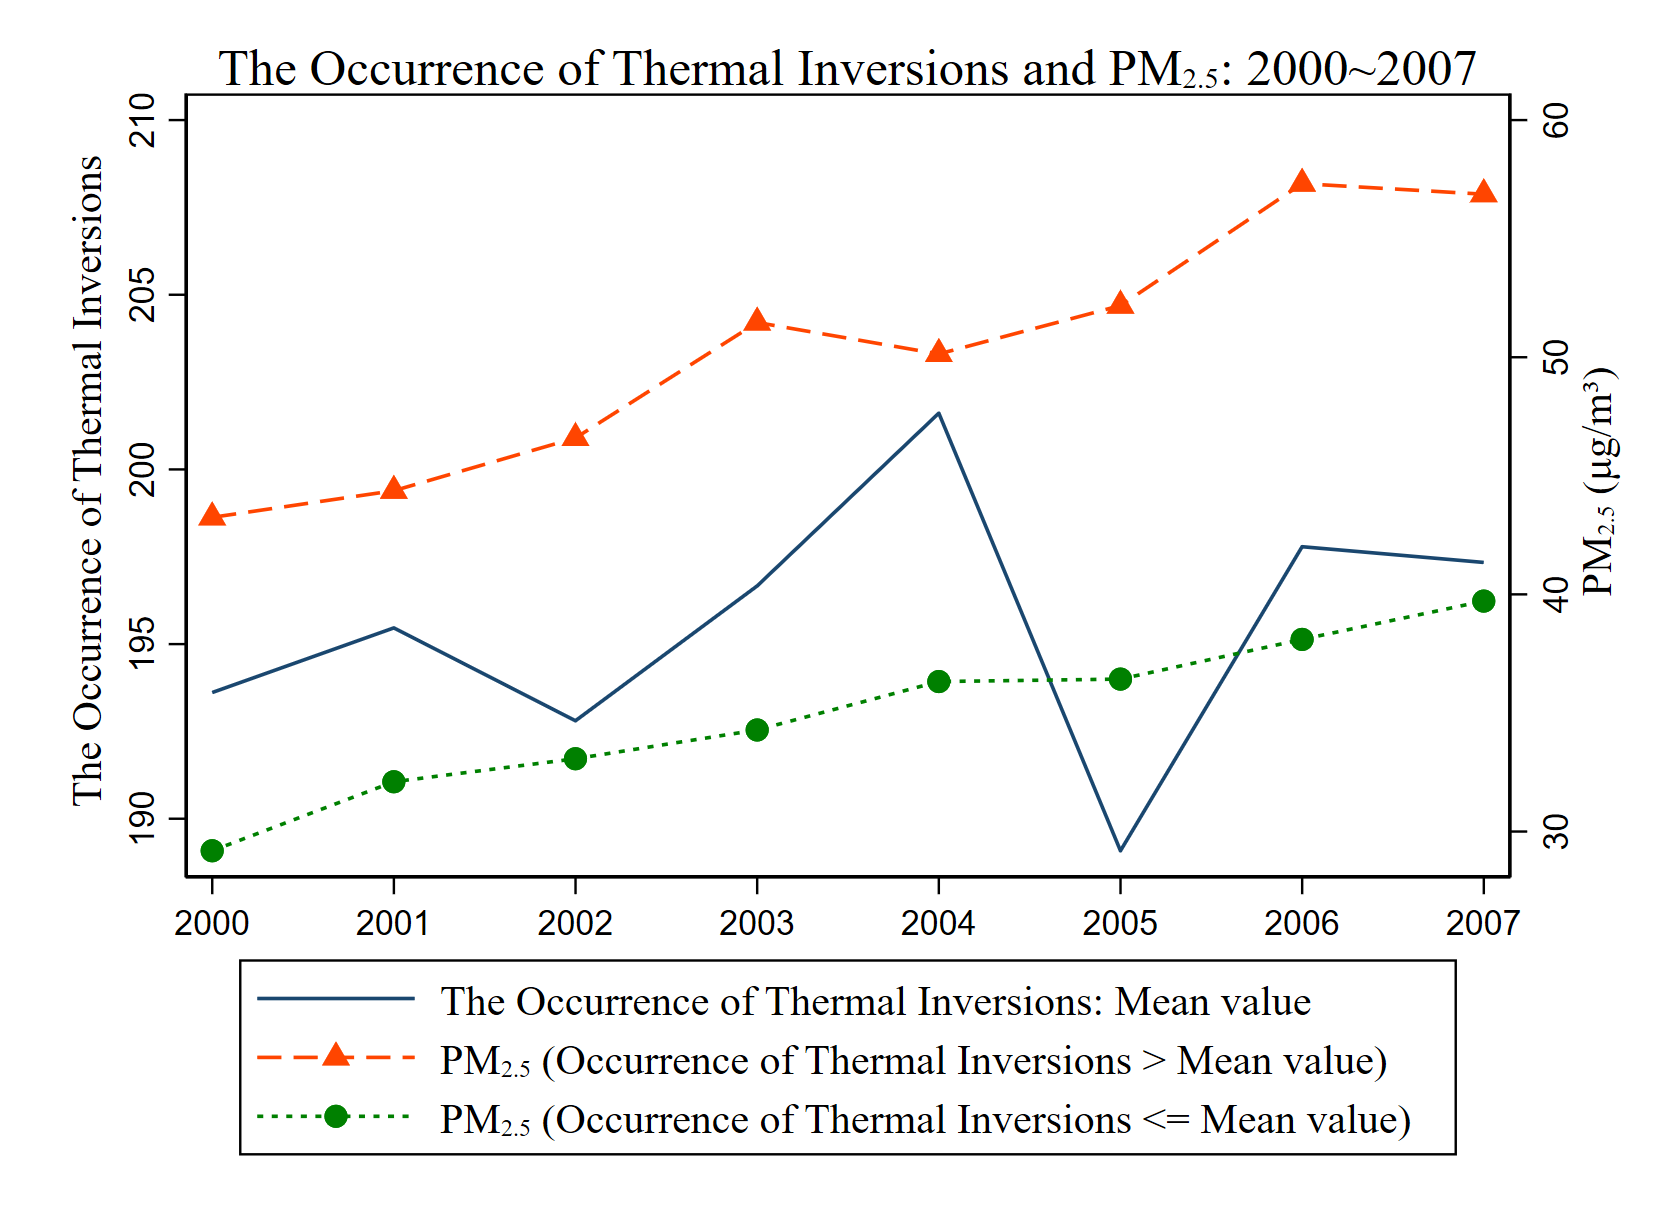
\includegraphics[width=\textwidth]{TI_PM25_2.eps}
    \end{minipage}
    \small
    \caption*{Notes: In the top panel, counties are divided into 90 quantiles according to annual days of thermal inversions. The horizontal axis indicates the annual days of thermal inversions in each quantile. The vertical axis indicates the mean value of $\rm PM_{2.5}$ concentrations in each quantile. The bottom panel shows the occurrence days of thermal inversions from year 1998 to 2007 and annual average $\rm PM_{2.5}$ concentrations in two thermal-inversion groups. Counties are divided into two groups. The blue dash line plots the average annual occurrence in days of thermal inversions over counties from year 1998 to 2007. The red dash line marked with triangle plots the average annual $\rm PM_{2.5}$ of counties whose occurrence of thermal inversions is above the average level and the green dash line marked with dots plots the average annual
    $\rm PM_{2.5}$ of counties whose occurrence of thermal inversions is below the average level.}
  \end{figure}

  \begin{figure}[H]\centering
    \centering
     \caption{Trends of PM2.5 and Exports}\label{fig:4}
      \begin{subfigure}[b]{.75\textwidth}
       \centering
        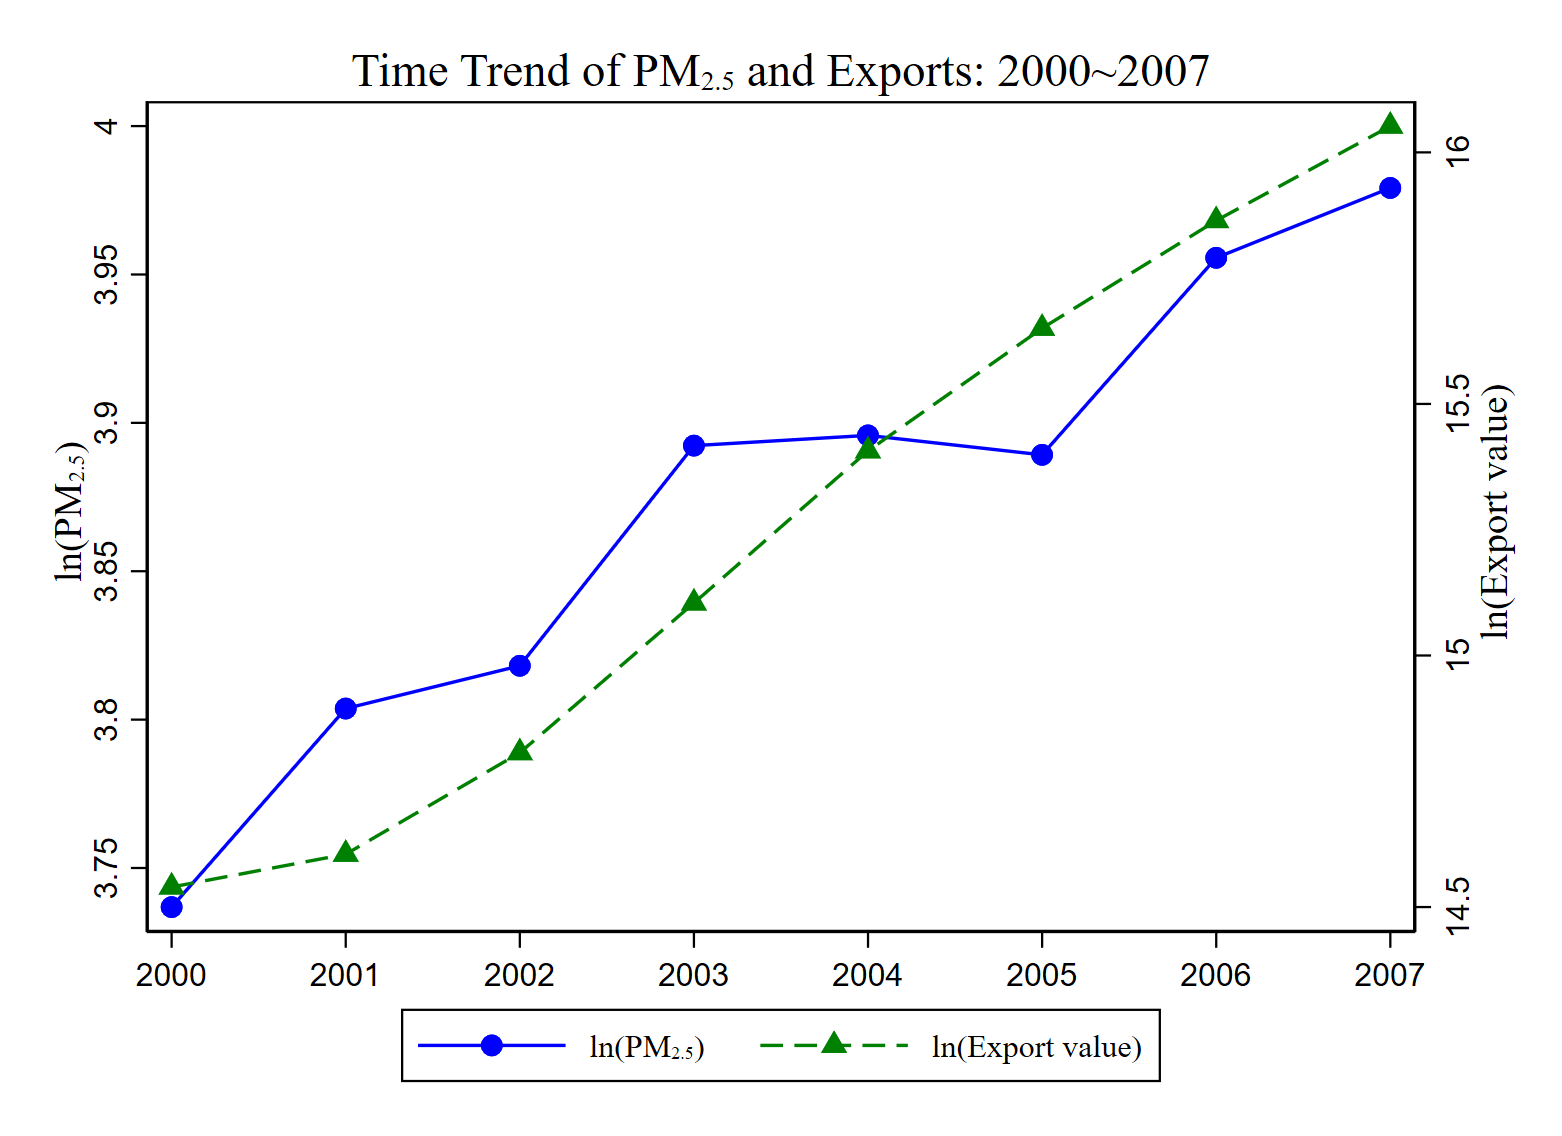
\includegraphics[width=\linewidth]{exp_pm25_trend.eps}
        \caption{}\label{fig:fig_4a}
        \end{subfigure}
%
         \begin{subfigure}[b]{.75\textwidth}
         \centering
         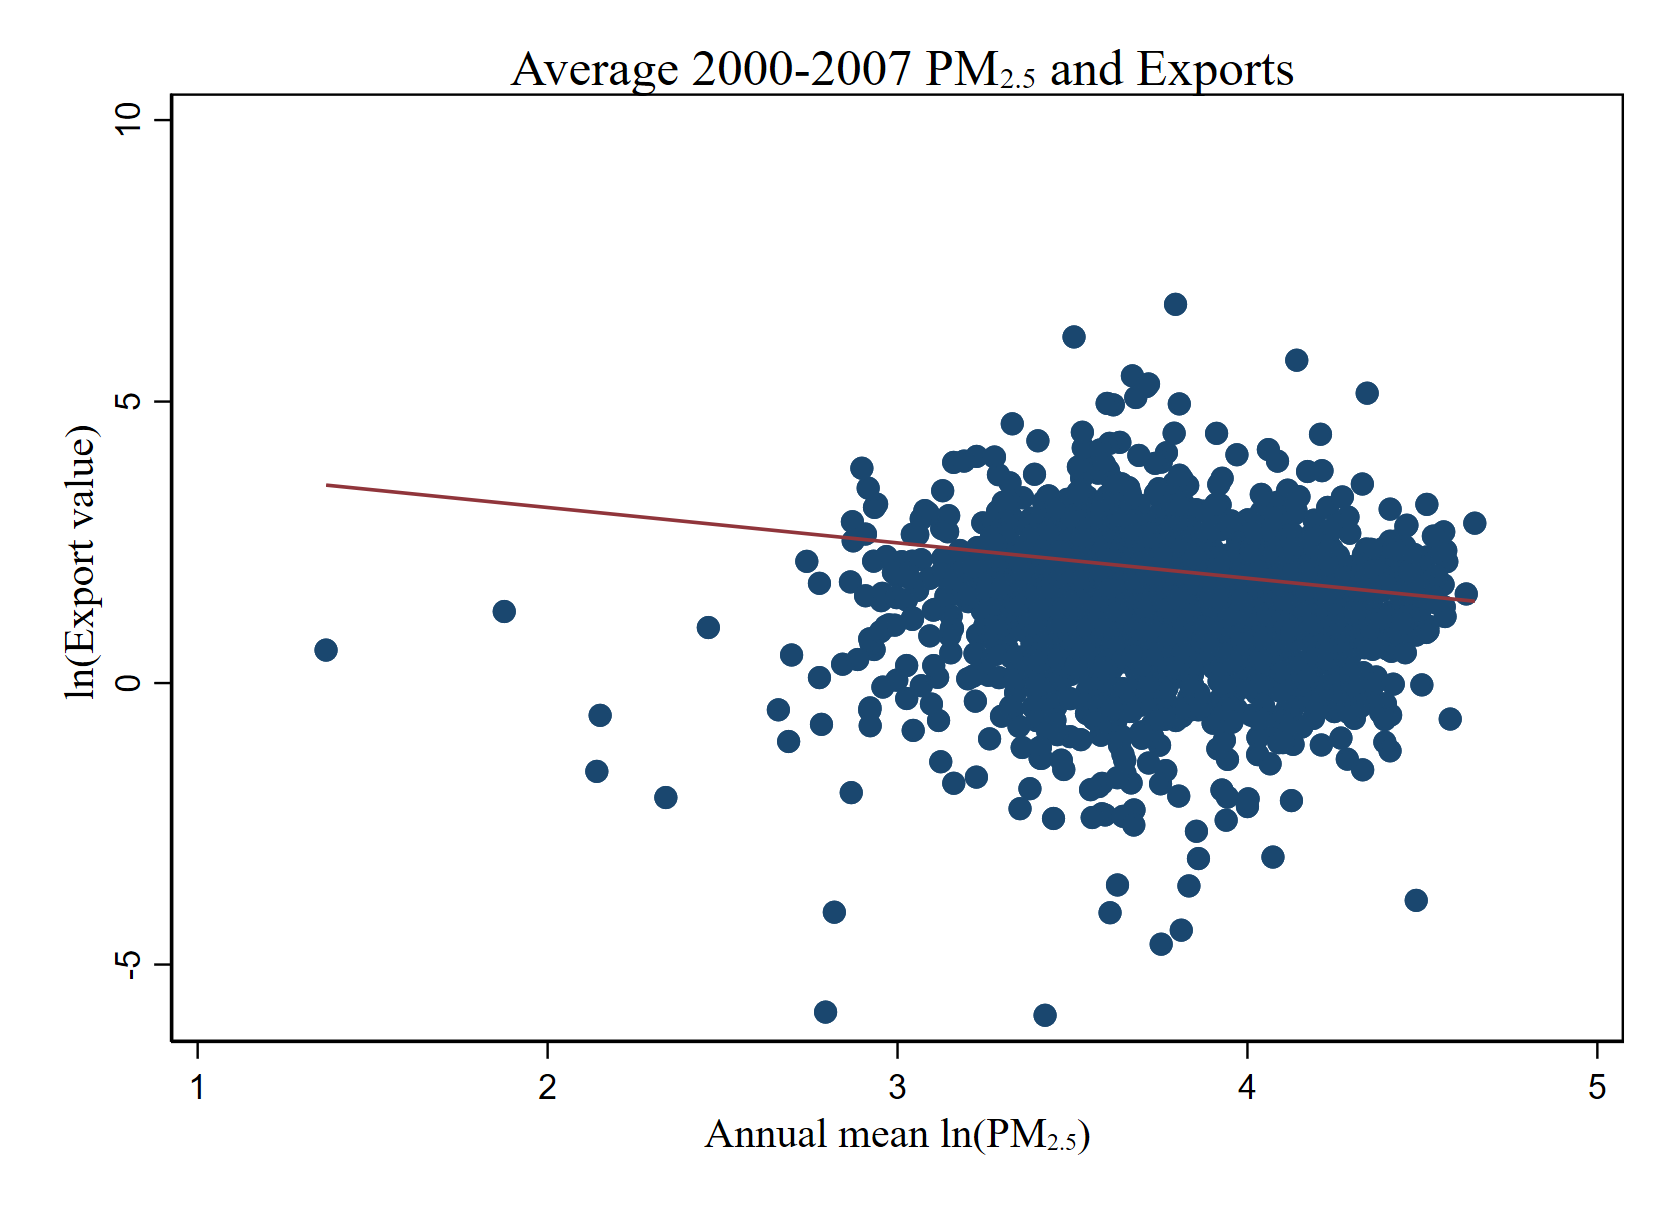
\includegraphics[width=\linewidth]{exp_pm25.eps}
          \caption{}\label{fig:fig_4b}
          \end{subfigure}
    \small
    \caption*{Notes: The top panel displays the trend of yearly average PM2.5 and exports from 2000 to 2007. The bottom panel displays the scatters of the county-level averages of PM2.5 and exports. The  fitted value line is drawn taking weights by the number of exporters in each county, in case a county with more exporters will be under-represented in the analysis.}
  \end{figure}
  \let\clearpage\relax
\end{document}